\documentclass[t,aspectratio=169]{beamer}
%\usetheme{Berkeley}
\usepackage{graphicx}
\usepackage{amsmath}
\usepackage[american]{circuitikz}
\usepackage{tcolorbox}

\title{Clase 25}
\subtitle{El transistor MOSFET no ideal II}
\author{Dr.-Ing. Juan José Montero Rodríguez}
\subject{Elementos Activos}
\institute{Escuela de Ingeniería Electrónica}
\date{Semestre II-2023}
\titlegraphic{
\includegraphics[height=8mm]{./figuras/logotec.pdf}}

\begin{document}

\begin{frame}{}
\maketitle
\end{frame}


\section{Efecto de substrato}
\begin{frame}{Efecto de substrato}

Recordando, la tensión de umbral $V_{TH}$ se define de acuerdo con la cantidad de carga necesaria para formar un canal.

\begin{itemize}
    \item La carga en la compuerta debe ser igual a la carga en el canal.
    \item En inversión, la concentración $n$ del canal es igual y opuesta a la concentración $p$ de la oblea.
\end{itemize}

\vspace{5mm}
Si ahora el substrato (B) tiene una tensión distinta de la tensión de la fuente (S), la cantidad de carga que aporta la tensión $V_{SB}$ \textbf{modifica la tensión de umbral}.

\begin{figure}[H]
    \centering
    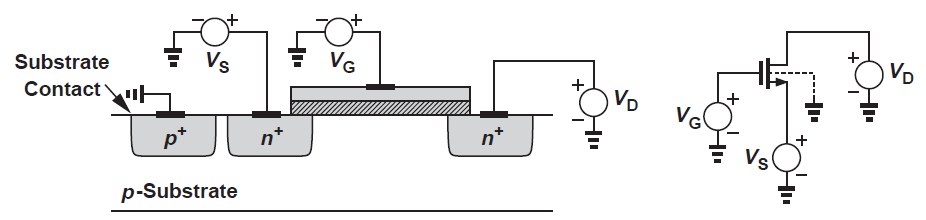
\includegraphics[width=0.8\textwidth]{figuras/body_effect.png}
\end{figure}

\end{frame}


\begin{frame}{Curva de transferencia con efecto de substrato}
\centering

\begin{figure}[H]
    \centering
    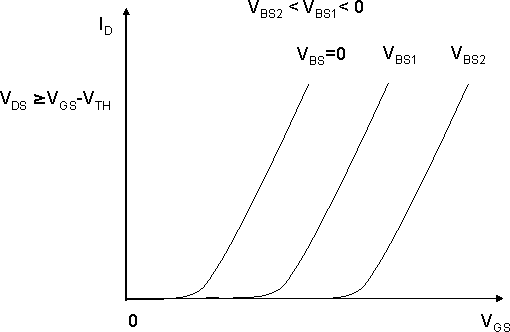
\includegraphics[width=9cm]{figuras/theffect.pdf}
\end{figure}

Un voltaje de substrato negativo con respecto al surtidor o bien un voltaje de surtidor positivo con respecto al substrato causan un aumento del voltaje de umbral
\end{frame}


\begin{frame}{Voltaje de umbral con efecto de substrato}
\begin{itemize}
	\item VBS$\neq$0 cambia el voltaje de umbral
	\item Se analiza aquí el caso de un NMOS
\end{itemize}

\[ V_{TH} = V_{TH0} + \gamma (\sqrt{2 \phi_F + V_{SB}} - \sqrt{ 2 \phi_F }) \]

Donde

\begin{itemize}
    \item $V_{TH0}$: Voltaje de umbral con $V_{SB} = 0$.
    \item $\gamma$: Coeficiente de efecto de substrato.
    \item $2\phi_{F}$: Potencial de superficie, requerido para inversión ($\phi_S = 2\phi_F$).
\end{itemize}

\vspace{5mm}\centering
$\gamma = \dfrac{\sqrt{2 q N_A \epsilon_{Si}}}{C_{ox}'}$

$\phi_F = V_t \cdot \ln \left( \dfrac{N_A}{n_i} \right)$

\end{frame}


\section{Ejemplo 1}
\begin{frame}{Ejemplo 1: Efecto de substrato}

Determine el valor de la corriente $I_D$ que fluye por el circuito, para un transistor ideal, y repita para un transistor con efecto de substrato.

\begin{columns}

\begin{column}{0.3\textwidth}

\begin{circuitikz}[arrowmos]
    \draw (0,0) node[nfet](M1){};
    \draw (M1.source) to[R,l=$R_S$] (0,-2);
    \draw (0,-2) node[ground]{};
    \draw (M1.bulk) -- (1,0);
    \draw (1,0) node[ground]{};
    \draw (-1,0) to[short,o-] (M1.gate);
    \draw (-1,0) node[left]{$V_G$};
    \draw (0,2) to[R,l=$R_D$] (M1.drain);
    \draw (0,2) node[vdd]{$V_{DD}$};
\end{circuitikz}

\end{column}

\begin{column}{0.35\textwidth}

\centering
\textbf{Parámetros de la tecnología}
\[ \mu_n C_{ox}' = 200\ \mu A/V^2 \]
\[ \dfrac{W}{L} = \dfrac{5}{0.18} \]
\[ V_{TH0} = 0.5\ V \]
\[ \gamma = 0.37\ V^{1/2} \]
\[ \phi_F = 0.3\ V \]

\end{column}

\begin{column}{0.35\textwidth}

\centering
\textbf{Parámetros del circuito}
\[ R_D = 220\ \Omega \]
\[ R_S = 330\ \Omega \]
\[ V_G = 2\ V \]
\[ V_{DD} = 3.3\ V \]

\end{column}

\end{columns}

\end{frame}


\begin{frame}{Solución 1: Efecto de substrato}

\begin{columns}

\begin{column}{0.3\textwidth}

\begin{circuitikz}[arrowmos]
    \draw (0,0) node[nfet](M1){};
    \draw (M1.source) to[R,l=$R_S$] (0,-2);
    \draw (0,-2) node[ground]{};
    \draw (M1.bulk) -- (1,0);
    \draw (1,0) node[ground]{};
    \draw (-1,0) to[short,o-] (M1.gate);
    \draw (-1,0) node[left]{$V_G$};
    \draw (0,2) to[R,l=$R_D$] (M1.drain);
    \draw (0,2) node[vdd]{$V_{DD}$};
\end{circuitikz}

\end{column}

\begin{column}{0.7\textwidth}

\textbf{Solución para un transistor ideal}
\[ I_D = \dfrac{1}{2} \mu_n C_{ox}' \dfrac{W}{L} (V_{GS} - V_{TH0})^2 \]
\[ V_G = 2\ V \]
\[ V_S = I_D R_S \]

\[ I_D = \dfrac{1}{2} (200\ \mu A/V^2) \left( \dfrac{5}{0.18} \right) \left(2\ V - I_D \cdot 330\ \Omega - 0.5\ V \right)^2 \]
\[ \boxed{I_D = 1.984\ mA} \]
\end{column}

\end{columns}
    
\end{frame}


\begin{frame}{Solución 1: Efecto de substrato}

\begin{columns}

\begin{column}{0.3\textwidth}

\begin{circuitikz}[arrowmos]
    \draw (0,0) node[nfet](M1){};
    \draw (M1.source) to[R,l=$R_S$] (0,-2);
    \draw (0,-2) node[ground]{};
    \draw (M1.bulk) -- (1,0);
    \draw (1,0) node[ground]{};
    \draw (-1,0) to[short,o-] (M1.gate);
    \draw (-1,0) node[left]{$V_G$};
    \draw (0,2) to[R,l=$R_D$] (M1.drain);
    \draw (0,2) node[vdd]{$V_{DD}$};
\end{circuitikz}

\end{column}

\begin{column}{0.7\textwidth}

\textbf{Solución para un transistor no ideal}
\[ V_{SB} = V_S - V_B = I_D R_S - 0 = I_D R_S \]
\[ V_{TH} = V_{TH0} + \gamma (\sqrt{2\phi_F + V_{SB}} - \sqrt{2\phi_F}) \]
\[ I_D = \dfrac{1}{2} \mu_n C_{ox}' \dfrac{W}{L} (V_{GS} - V_{TH})^2 \]

Las ecuaciones anteriores se combinan:
\[ I_D = \dfrac{1}{2} \mu_n C_{ox}' \dfrac{W}{L} (V_{GS} - (V_{TH0} + \gamma (\sqrt{2\phi_F + V_{SB}} - \sqrt{2\phi_F})))^2 \]

Donde
\[ V_{GS} = V_G - V_S = 2\ V - I_D R_S \]

\end{column}

\end{columns}
    
\end{frame}



\begin{frame}{Solución 1: Efecto de substrato}

La ecuación completa es:
\begin{multline*}
I_D = \dfrac{1}{2} (200\ \mu A/V^2) \left( \dfrac{5}{0.18} \right) \times \\ 
\left(2\ V - I_D \cdot 330\ \Omega - (0.5\ V + (0.37\ V^{1/2})(\sqrt{0.6\ V + I_D \cdot 330\ \Omega} - \sqrt{0.6\ V})) \right)^2
\end{multline*}

Resolviendo por SHIFT+SOLVE:
\[ \boxed{I_D = 1.773\ mA} \]

La tensión de umbral efectiva es:
\[ 0.5\ V + (0.37\ V^{1/2})(\sqrt{0.6\ V + I_D \cdot 330\ \Omega} - \sqrt{0.6\ V}) \]
\[ \boxed{V_{TH} = 0.616\ V} \]
    
\end{frame}


\section{Subumbral}
\begin{frame}{Región de subumbral}

Corriente de drenador en la región de subumbral: $V_{GS} < V_{TH}$

\begin{columns}

\begin{column}{0.7\textwidth}

\begin{tcolorbox}
\[ I_D = I_{D0} \cdot e^{\dfrac{(V_{GS} - V_{TH})}{mV_t}} = I_{D0} \cdot e^{\dfrac{(V_{GS} - V_{TH}) \ln 10}{S}} \]
\end{tcolorbox}

\end{column}

\begin{column}{0.3\textwidth}

\[ m = 1 + \dfrac{C_{dep}}{C_{ox}} \]

C\textsubscript{dep} : capacitancia de agotamiento de substrato

C\textsubscript{ox} : capacitancia de compuerta

\end{column}

\end{columns}

Se define la pendiente de subumbral:
\[ S = \left[\dfrac{d(\log I_{DS})}{dV_{GS}}\right]^{-1} = \ln 10 \cdot V_t \cdot m \]

\centering A T=300K, S=80..85 mV/dec; a T=100$^\circ$ C, S=100mV/dec


\end{frame}


\begin{frame}{Corriente de subumbral}
\centering
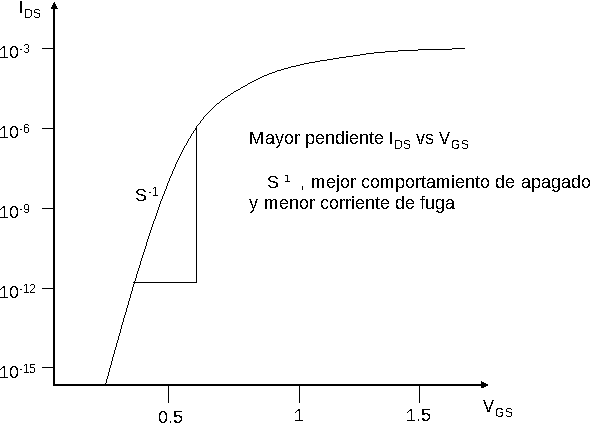
\includegraphics[width=10cm]{figuras/subth.pdf}
\end{frame}


\section{Ejemplo 2}
\begin{frame}{Ejemplo 2: Región de subumbral}

Para un MOSFET de 180 nm se ha estimado que la corriente en el punto de encendido, justo cuando $V_{GS} = V_{TH}$, es aproximadamente:
\[ I_{D0} = I_D (V_{GS}=V_{TH}) \times \dfrac{W}{L} \approx 0.1 \mu{}A \times \dfrac{W}{L} \]

\begin{itemize}
    \item Determine la corriente $I_D$ para un transistor de dimensiones $W/L=5/0.18$ cuando la tensión $V_{GS}=0.40\ V$.
    \item Utilice Python para graficar la corriente $I_D$ en función de $V_{GS}$ en el intervalo $0 < V_{GS} < V_{TH}$. Grafique en escala semilogarítmica.
    \item Mida de la gráfica el valor de la pendiente de subumbral.
\end{itemize}
    
\end{frame}


\begin{frame}{Solución 2: Región de subumbral}

   
\end{frame}


\section{Referencias}
\begin{frame}{Lecturas recomendadas}

\begin{itemize}
    \item Razavi, B. (2013). Fundamentals of microelectronics. Chapter 6: Physics of MOS transistors, 2nd ed., pp. 288-295, Wiley.
\end{itemize}

\end{frame}

\end{document}
